\subsection{temperature} 
the temperature was measured every 2 minutes over the course of 1 week. the minimal temperature was reached on monday 8-12-2022 with a degree of 11°C on sensor 12 the maximum temperature was reached on wednseday 11-12-2022 with a degree of 21°C on sensor 5.\\ 
\begin{figure}[hbt!] 
\begin{subfigure}{0.5\textwidth} 
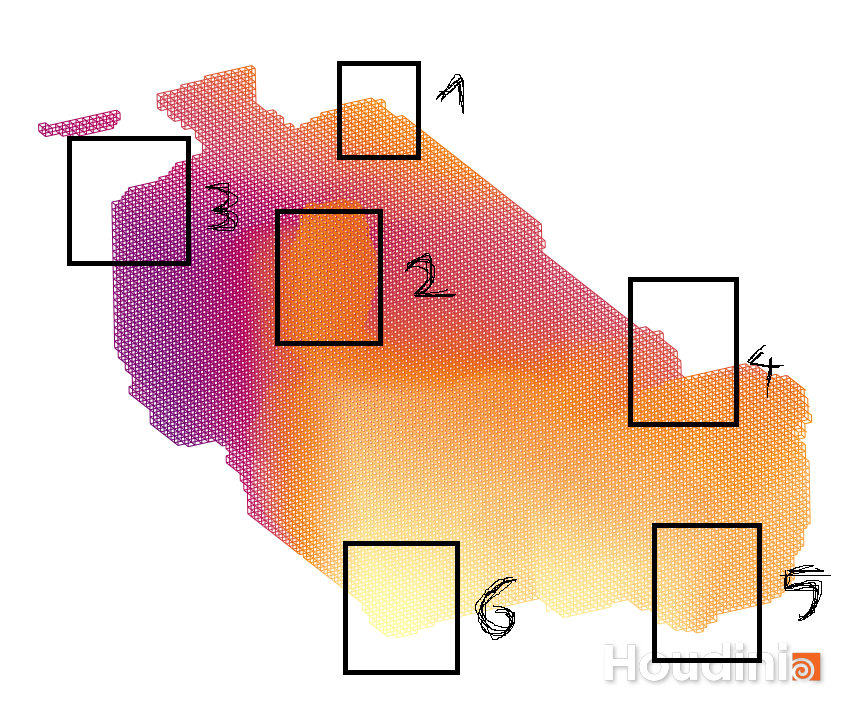
\includegraphics[width=0.99\linewidth]{reports/current_report/images/max_temperature.png}  
\caption{max temperature}  
\end{subfigure} 
\begin{subfigure}{0.5\textwidth} 
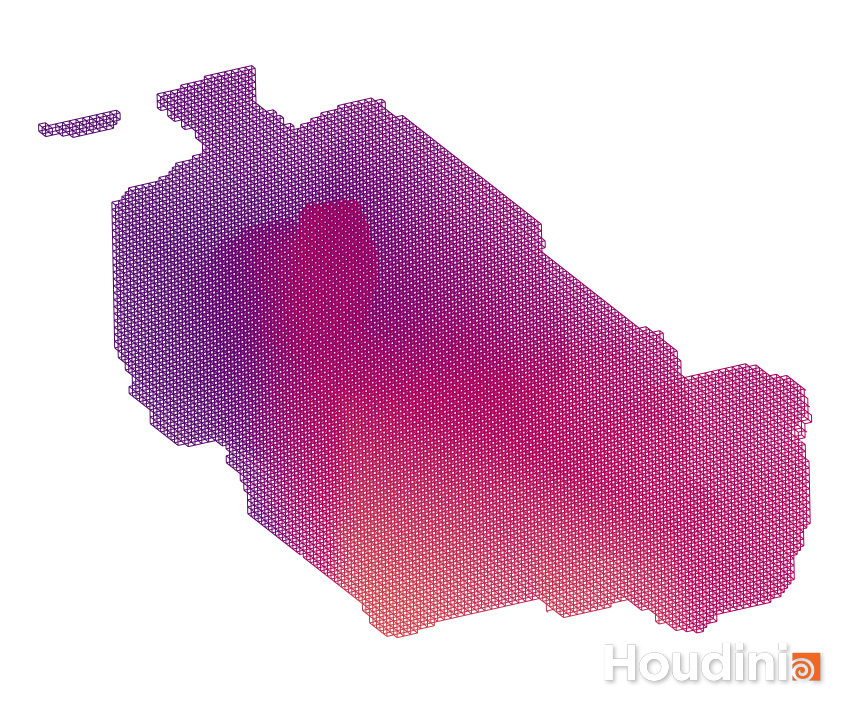
\includegraphics[width=0.99\linewidth]{reports/current_report/images/min_temperature.png}  
\caption{min temperature}  
\end{subfigure} 
\caption{comparison between the minimum and maximum  temperature}  
\end{figure} 
\FloatBarrier 
the average temperature during week 1 (5th of December until the 12th of December) was 17 °C. \\an overview of the temperatureimages can be seen here:\begin{figure}[hbt!] 
\centering 
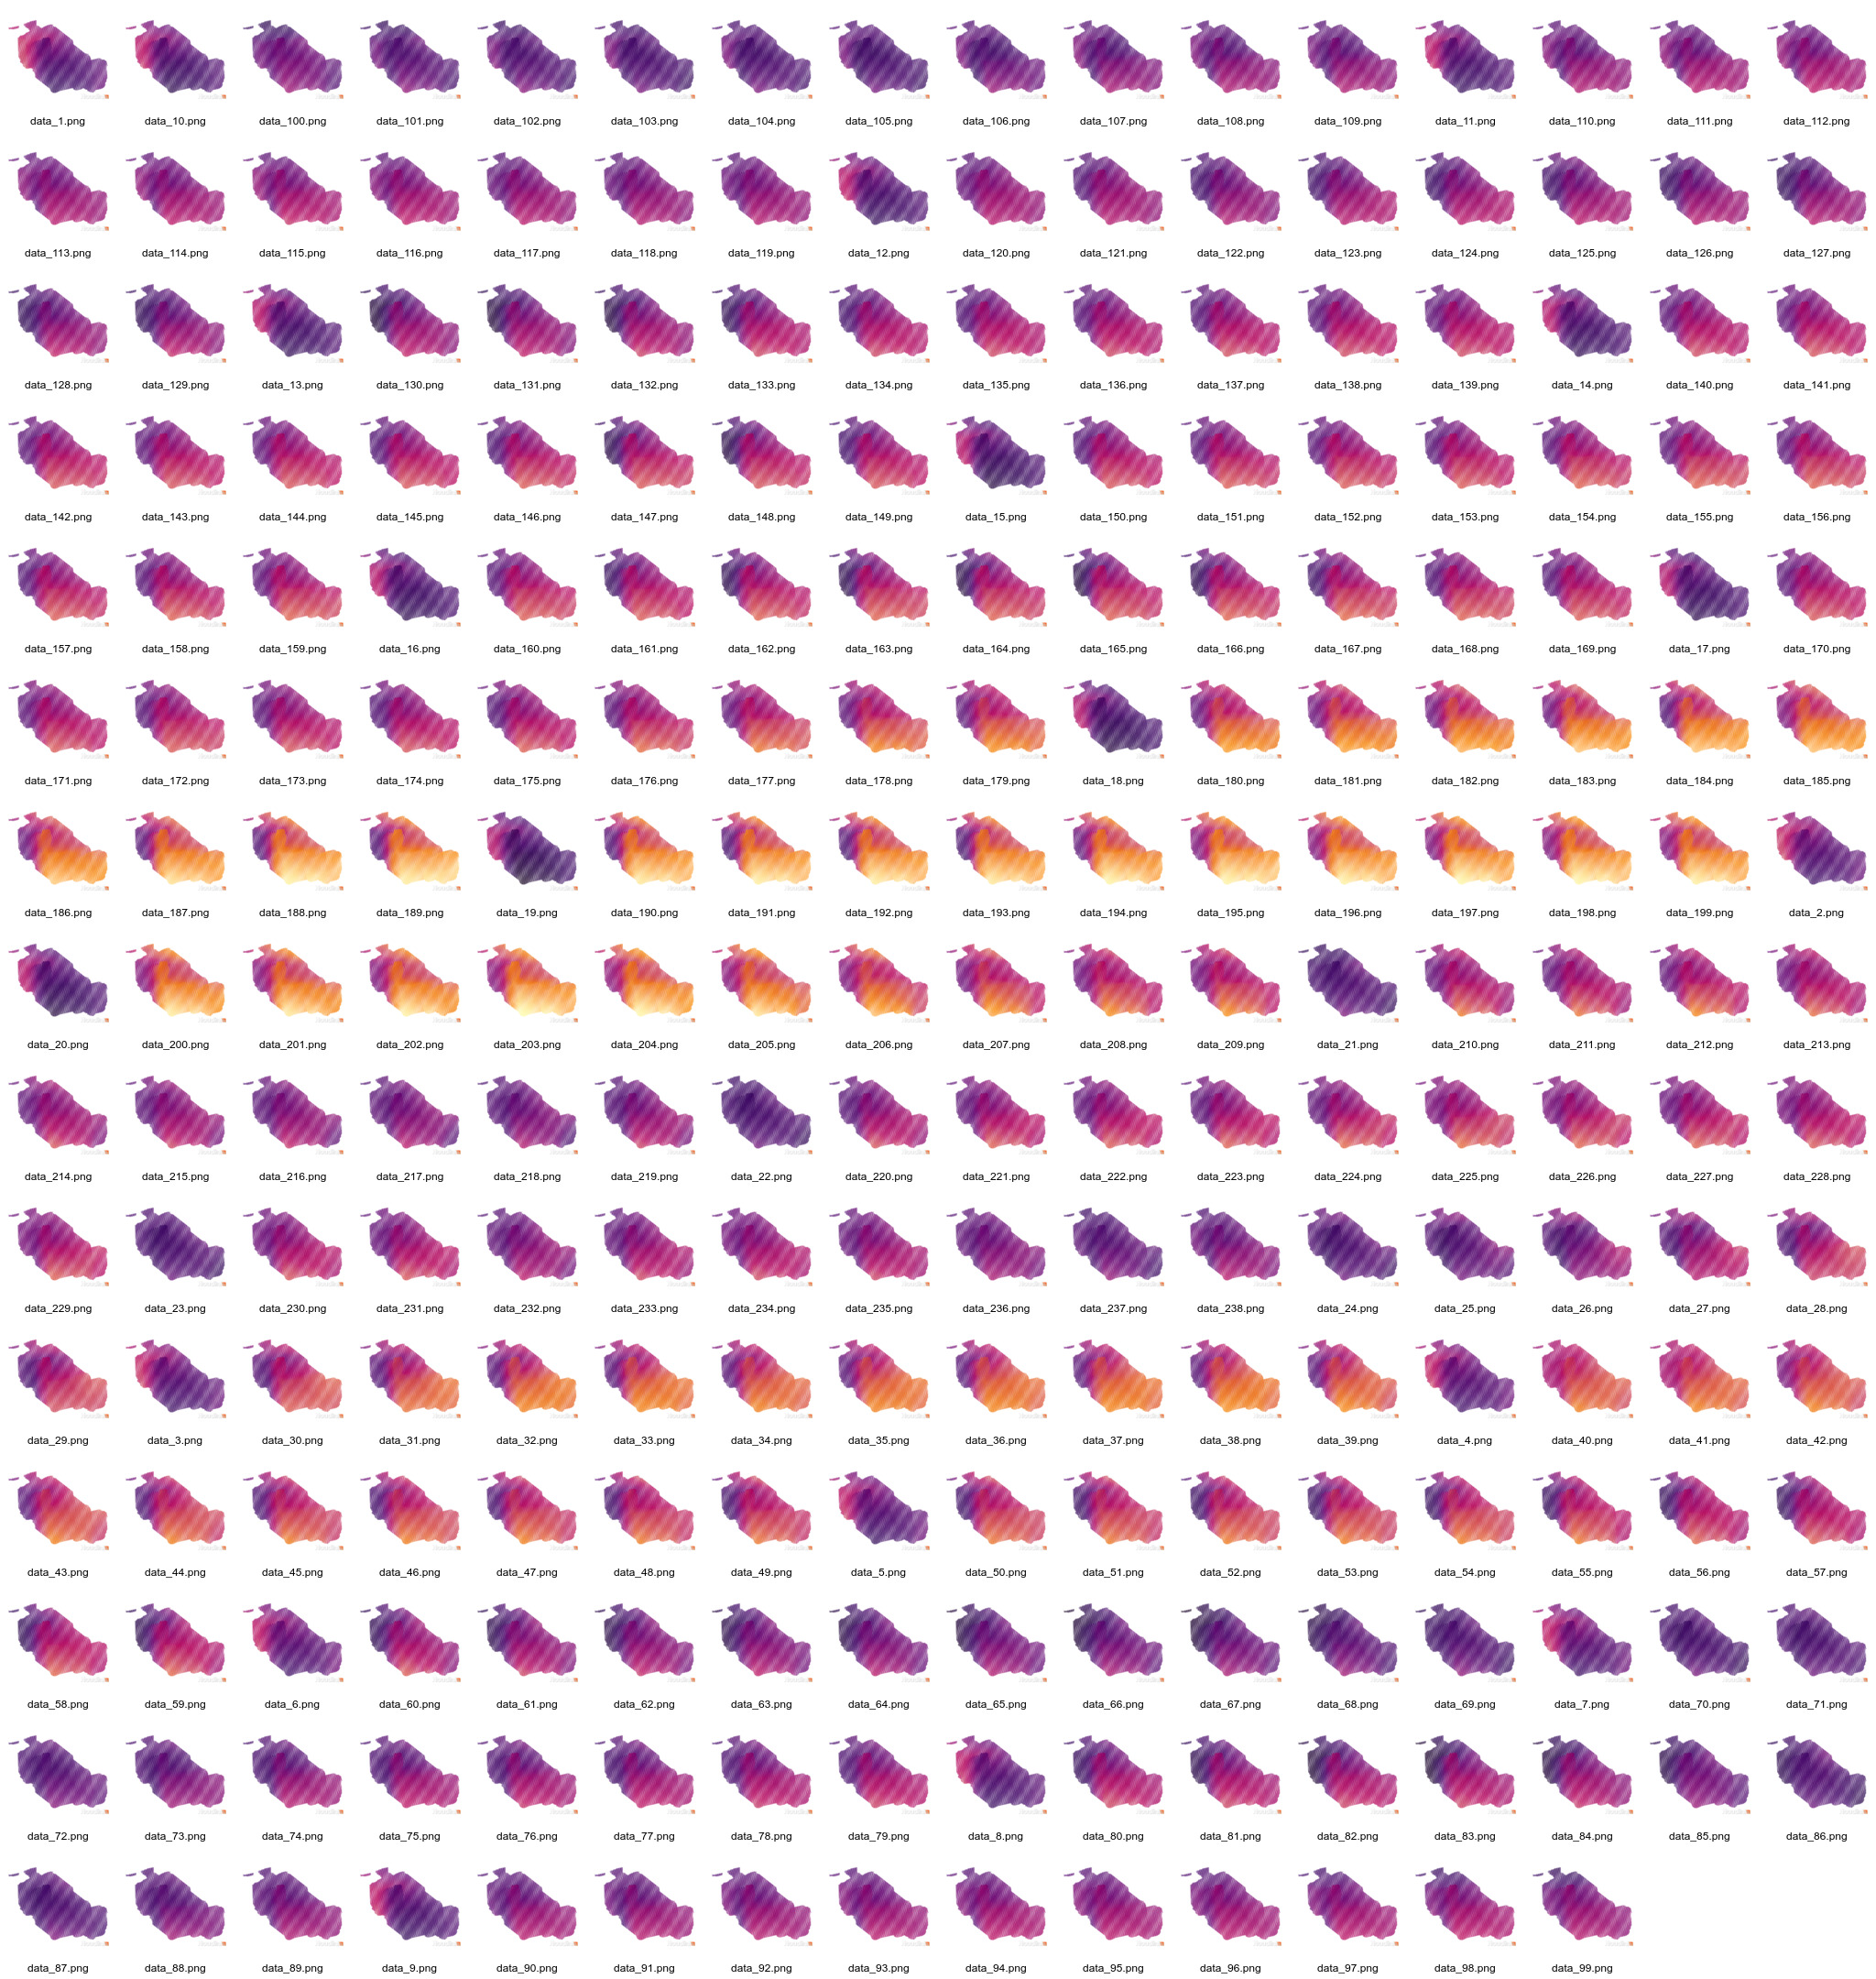
\includegraphics[width=\textwidth]{reports/current_report/images/montage_temperature.jpg}  
\caption{mosaic of the temperature measuruments} 
\end{figure} 
\FloatBarrier 
a live visualisation of the data can be seen \href{https://data.hasdata.xyz/}{here}. an animation of the week's data can be seen \href{https://data.hasdata.xyz/}{here}. 